\chapter{Biomarker}
\label{chapter:intro}
\section{遺生物標記(Biomarker)介紹}
在醫學上通常是指在血液中的某種蛋白質,通過測量它,可以反映出某種疾病是否出現或嚴重程度。


\label{sec:background}
\section{血漿(phospho-tau,P-tau)與阿茲海默氏病(Alzheimer disease,AD)}

具有輕微認知症狀(例如記憶力下降)的患者是否患有前期或臨床前阿茲海默氏病(Alzheimer disease,AD)並在不久的將來發展為 AD 癡呆仍然是臨床醫生面臨的挑戰。這項任務對於正確和早期的 AD 診斷、開始對AD症治療、規劃未來以及希望很快開始改善疾病的治療都至關重要。

儘管在 AD 和進展為 AD 癡呆的生物標誌物方面取得了令人矚目的進展,但這些方法大多數都是侵入性、高成本和有限的,可用性限制了它們的使用數量和限制只能在高度專業化的醫學中心。
 
隨著最近基於血液的生物標誌(在醫學上通常是指在血液中的某種蛋白質,通過測量它,可以反映出某種疾病是否出現或嚴重程度)的發展,出現了一個可能的轉折點,這使就在血漿中,尤其是血漿 P-tau181 和 P-tau217,在區分 AD 癡呆與其他神經退行性疾病方面表現出特別高的正確性。在有認知障礙的患者的臨床檢查中,由於 AD 病因的多因素性質及其異質的臨床表現,只使用血漿本身不太可能實現最高的潛在預測準確性.因此需要使用血漿與其他測量相結合,以對AD 產生最準確的預測,並為早期診斷建立非侵入性、成本效益高且易於獲得的最佳診斷算法。


\section{用P-tau217預測 4 年內 AD }
\begin{figure}[H]
	\centerline{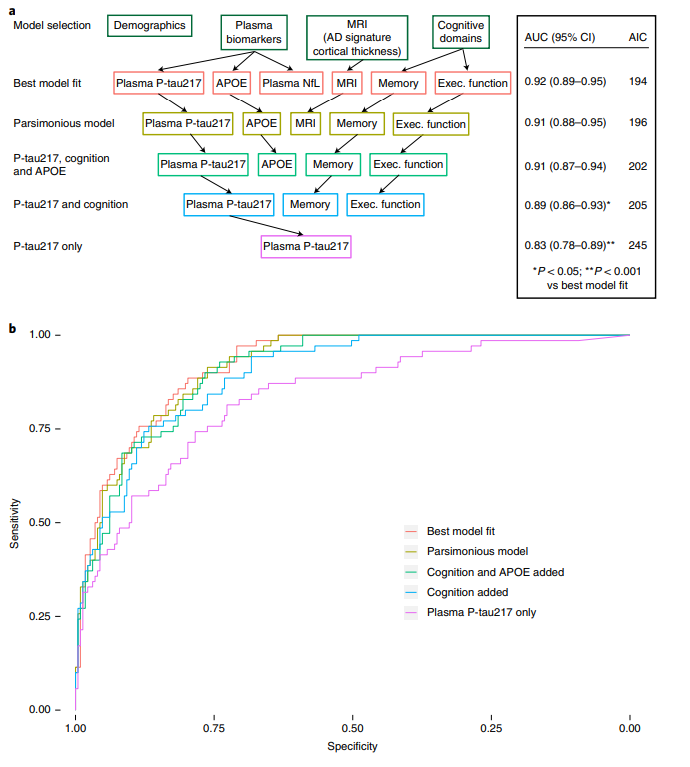
\includegraphics[height=8cm]{pic/AD217.PNG}}
	\caption{P-tau217預測 4 年內 AD圖}
	\label{fig:AD217}
\end{figure}
最佳模型為包括預測因子血漿 P-tau217、APOE 等位基因、執行功能、記憶功能、磁共振成像(magnetic resonance imaging,MRI)和血漿 NfL.該模型的 AUC 為 0.92(95\% 置信區間 (Confidence interval,CI) 0.89–0.95);去除血漿 NfL和MRI,準確度 (AUC = 0.91, 95\% CI 0.87–0.94)。


\section{用P-tau181預測 4 年內 AD }
\begin{figure}[H]
	\centerline{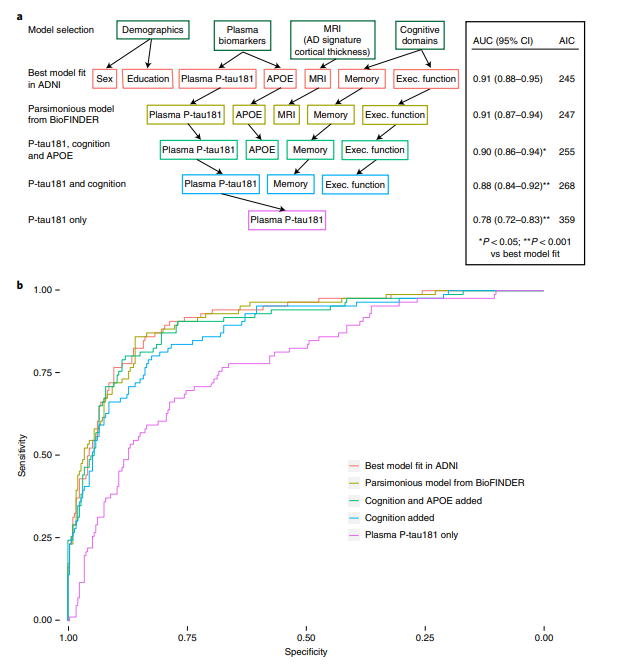
\includegraphics[height=8cm]{pic/AD181.PNG}}
	\caption{P-tau181預測 4 年內 AD圖}
	\label{fig:AD181}
\end{figure}
最佳模型為包括預測因子血漿 P-tau181、APOE 等位基因、執行功能、記憶功能、MRI,該模型的 AUC 為 0.91 95\% CI 0.88–0.95);去除MRI,準確度也還有 (AUC = 0.90, 95\% CI 0.86–0.92)。


\section{血漿用於預測AD結論}
預測主要在 4 年內進展為 AD 癡呆,雖然單獨血漿 P-tau 可以在 4 年內準確預測 AD 癡呆(AUC = 0.83),但當它與APOE 基因型和認知測試相結合時,準確性的提高為顯著(AUC = 0.91)。就算加入能最為準確預測AD的MRI準確性的提高也只有而已(AUC = 0.92)。

使用血液的生物標誌,能避免運用MRI與脊髓抽取等對人體清害較大的方法進行AD的預測檢驗,只要進行抽血並配合執行力與記憶力功能等認知測驗,也能擁有寮好的的預測結果,幫助醫生在臨床上進行診斷。

